This chapter describe the evolution of frame format proposed in \ref{ch:proposal}. Also, describe the reason
 of each change based on better understand of need of others team and the problems in the development


\section{MAC Frame Construction}
%TODO Le
The proposed frame format in \ref{ch:proposal} had all the necessary fields and some removed to keep the model simple
The final frame format is  shown in \ref{tab:finalFrame}.
The figure \ref{fig:stateMachine} is the final state machine used to shows how the receiver will work

\begin{table}
\begin{tabular}{| c | c | c | c | c | c | c | }
  \hline                       
  Frame Type & Receiver UE & Sender UE & Data Size & Header CRC & Data & Data CRC\\
  \hline
	1 Byte & 1 Byte & 1 Byte & 1 Byte & 1 Byte & 1 to 234 Bytes & 1 Byte\\
  
  \hline  
\end{tabular}
 \caption{Final Frame Format}
	\label{tab:finalFrame}
\end{table}

\section{Transmission and reception process}
%Rebecca

% so I am going to be describing the state machine essentially....was going to do this but I might go and write the intro frist to have a beter idea of what is going on.


\subsection {Routing}

\section{Frame Types descriptions}
%Renato


%RGB 253 254 202
\begin{figure}[p]
    \centering
    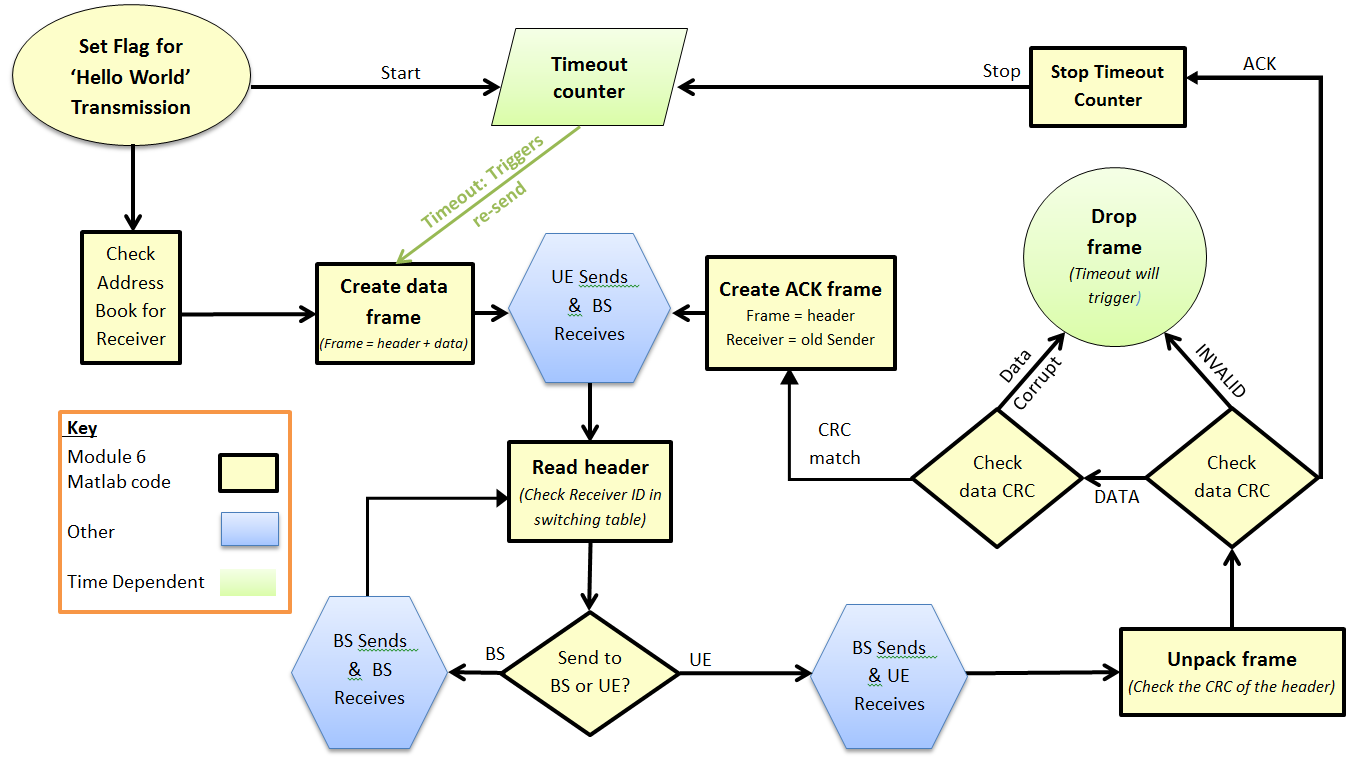
\includegraphics[width=0.8\textwidth]{State_Machine_yellow.PNG}
    \caption{State Machine of the transmission of a package }
    \label{fig:stateMachine}
\end{figure}

\begin{figure}[p]
    \centering
    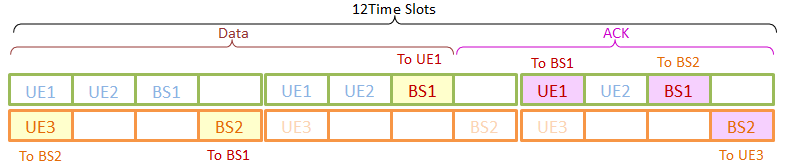
\includegraphics[width=0.8\textwidth]{ACK_timeout_long.PNG}
    \caption{Diagram of an example of the longest time between a UE transmitting frame of data and receiving the corresponding ACK}
    \label{fig:ACKtimelong}
\end{figure}

\begin{figure}[p]
    \centering
    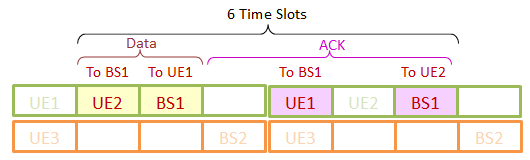
\includegraphics[width=0.8\textwidth]{ACK_timeout_short.PNG}
    \caption{Diagram of the shortest time between a UE transmitting a frame of data and receiving the corresponding ACK}
    \label{fig:ACKtimeshort}
\end{figure}

\begin{figure}[p]
    \centering
    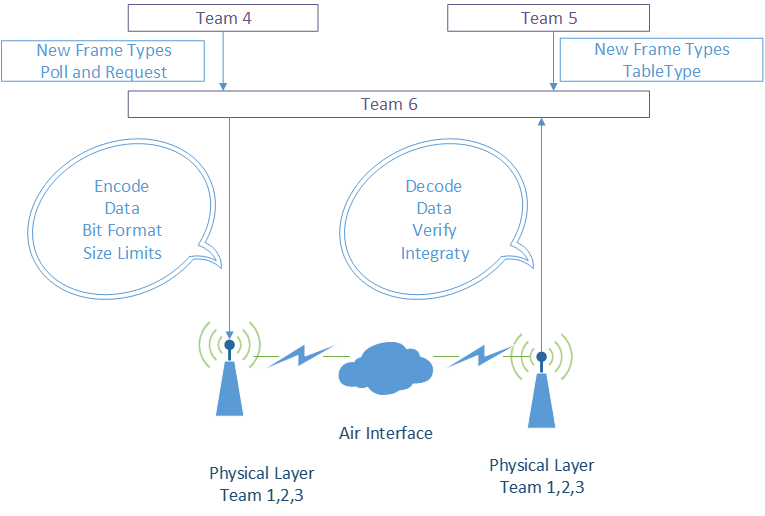
\includegraphics[width=0.8\textwidth]{Interface_diagram.PNG}
    \caption{Diagram of how Module 6 interfaces with the rest of the network}
    \label{fig:Interface}
\end{figure}